\chapter{Principles of Nuclear Magnetic Resonance Imaging}
\label{chap:Theory}

\begin{abstract}
	\lipsum[1]
\end{abstract}
\newpage

\section{Source of the NMR Signal}
\label{sec:theory_source_of_nmr}

\subsection{Nuclear Spin}
\label{subsec:theory_nuclear_spin}
The \ac{NMR} signal arises from the interaction between the atomic nucleus and an external magnetic field. These atomic nuclei poses intrinsic properties, mass ($m$), charge ($q$) and spin ($I$). Spin is a quantum mechanical property and as such, can only take values of half integers or integers. Nuclear spin is dictated by the sum of the constituent particles of the nucleus, protons and neutrons, each of which posses their own spin of either $\sfrac{1}{2}$ or $-\sfrac{1}{2}$. The additive nature of nuclear spin means that pairs of nucleons can cancel out leaving the nucleus with zero net spin, this happens when the nuclei contains and even number of protons and neutrons. If the nuclei contains an odd number of both protons and neutrons, it will have a positive integer nuclear spin whereas if the nuclei has an odd number of protons or neutrons, it will have a half integer spin. 

%\subsection{Nuclear Magnetisation}

The spin angular momentum, $\mathbf{J}$ of a nucleus of spin $I$ is given by
\begin{equation}
\left|\mathbf{J}\right| = \hbar \sqrt{I\left(I+1\right)}
\label{eq:theory_angular_momentum}
\end{equation}
where $\hbar$ is the reduced Plank's constant, $\sfrac{h}{2\pi}$. As the nucleus is charged and rotating, it gives rise to a current and therefore a magnetic moment $\mathbf{\mu}$,
\begin{equation}
\mathbf{\mu}=\gamma \mathbf{J}
\label{eq:theory_magnetic_moment}
\end{equation}
where $\gamma$ is the gyromagnetic ration for the nucleus, a constant which depends on the charge and mass of the nucleus. Table \ref{tab:theory_isotope_spin_gmr} shows the gyromagnetic ratio ($\gamma$) and nuclear spin ($I$) of common \ac{NMR} sensitive isotopes \cite{harris_n.m.r._1976, bernstein_handbook_2004, westbrook_mri_2015}. Due to its relatively high gyromagnetic ratio, compared to other nuclei used for \ac{NMR}, and relative abundance in the body, \ce{^{1}H}, a single proton, is most commonly used for \ac{MRI}.

\begin{table}[H]
	\centering
	\begin{tabular}{lccc}
		\hline
		Isotope            & Spin & $\gamma$ (MHzT$^{-1}$)                     & Sensitivity Relative to \ce{^{1}H}     \\ \hline
		\ce{^{1}H}         & $\sfrac{1}{2}$  & 42.58                                      & 1                                      \\
		\ce{^{2}H}         & $1$    & 6.54                                       & 0.0097                                 \\
		\ce{^{13}C}        & $\sfrac{1}{2}$  & 10.71                                      & 0.016                                  \\
		\ce{^{19}F}        & $\sfrac{1}{2}$  & 40.05                                      & 0.83                                   \\
		\ce{^{23}Na}       & $\sfrac{3}{2}$  & 11.27                                      & 0.093                                  \\
		\ce{^{31}P}        & $\sfrac{1}{2}$  & 17.25                                      & 0.066                                  \\ \hline
	\end{tabular}
	\caption{Common \ac{NMR} isotopes, their nuclear spin, gyromagnetic ratio and sensitivity, relative to \ce{^{1}H}.}
	\label{tab:theory_isotope_spin_gmr}
\end{table}

\subsection{Application of an External Magnetic Field}
If we consider the hydrogen nuclei in a sample of tissue, the number of possible eigenstates for a nucleus of nuclear spin $I$ is $\left(2I + 1\right)$. This means that for the \ce{^{1}H} nuclei in our sample, where $I=\sfrac{1}{2}$, we can observe two possible eigenstates, $\left| + \sfrac{1}{2} \right \rangle$ and $\left| - \sfrac{1}{2} \right \rangle$ often written as $\left|  \uparrow \right \rangle$ and $\left|  \downarrow \right \rangle$. In the absence of an external magnetic field, these states are degenerate as they have the same energy, however, if we move our sample into a static external magnetic field along the $z$-axis, $B_0$, the energy levels separate.\\
The $z$-component of the magnetic moment is defined by,
\begin{equation}
\mu_z=\gamma \hbar \mu_I
\label{eq:theory_longitudinal_magnetic_moment}
\end{equation}
where $m_I$ are the possible spin quantum numbers of the nucleus. For our proton system with spin $\sfrac{1}{2}$, $\mu_z$ is given by
\begin{equation}
\mu_z = \pm \frac{1}{2}\gamma\hbar.
\end{equation}
The spins can either be aligned parallel to the external magnetic field in the lower energy of the two eigenstates, also known as spin up, or anti-parallel to the magnetic field in the higher energy eigenstate, spin down. The energy difference between these two eigenstates is given by,
\begin{equation}
\Delta E = \gamma \hbar B_0.
\label{eq:theory_zeeman}
\end{equation}
For an ensemble of spins in an external magnetic field, there will be an imbalance between the populations of each state with more spins occupying the lower of the two energy states. The net magnetisation of the sample is simply the sum of the constituent spins and as such, the application of an external magnetic field leads to the sample gaining a net magnetisation vector aligned with $B_0$. This effect is very small, the magnitude of the imbalance between eigenstates can be derived from Boltzmann statistics and is given by,
\begin{equation}
\frac{N_{\uparrow}}{N_{\downarrow}} = \exp \left(\frac{\Delta E}{k_B T}\right),
\label{eq:theory_boltzman}
\end{equation}
where $N_{\downarrow}$ and $N_{\uparrow}$ are the the number of spins aligned with and against $B0$ respectively, $k_B$ is Boltzmann's constant and $T$ is the temperature of the system. This means that for a sample of biological tissue at body temperature in a 3T magnetic field, the population difference is very small at approximately three parts per million. Although this measurable proportion is very small, it can be detected due to the high density of protons in the tissue. The signal can also be increased by the application of a stronger $B_0$.

\subsection{Precession}
%The nuclear magnetic moment always has a transverse component as from equations \eqref{eq:theory_angular_momentum}, \eqref{eq:theory_magnetic_moment} and \eqref{eq:theory_longitudinal_magnetic_moment} we can see $\left| \mathbf{\mu} \right| > \mu_z$, and therefore the magnetic moment cannot exactly align along the $z$-axis. This misalignment between $\mathbf{\mu}$ and $B_0$ causes $\mathbf{\mu}$ to precess around $B_0$ at an angular frequency $\omega_0$, known as the Larmor frequency and is given by,
%\begin{equation}
%\omega_0=\gamma B_0.
%\end{equation}

Classically, if a magnetic moment, M, is placed into an external magnetic field, B, it will experience a torque, $\tau$, proportional to change in angular momentum and thus induce a rotation.
\begin{equation}
\mathbf{M \times B} = \frac{d\mathbf{J}}{dt} = \tau
\label{eq:theory_classical_torque}
\end{equation}
From \eqref{eq:theory_magnetic_moment} the quantum equivalent of \eqref{eq:theory_classical_torque} is the standard form of the Bloch equation\cite{bloch_nuclear_1946},
\begin{equation}
\frac{d\mathbf{\mu}}{dt} = \gamma \mathbf{\mu \times B}
\label{eq:theory_bloch_standard}
\end{equation}
This equation states that if the magnetic moment, $\mu$ is not aligned with the external magnetic field, $\mathbf{B}$, it will precess about $\mathbf{B}$. The frequency of this precession, $\omega_0$ is known as the Larmor frequency and is given by substituting Bohr's frequency condition of the Planck relation ($\Delta E = \hbar \omega $) into \eqref{eq:theory_zeeman},
\begin{equation}
\omega_0=\gamma B_0,
\label{eq:theory_larmor}
\end{equation}
Nuclei with a positive gyromagnetic ratio precess clockwise, whereas nuclei (and the electron) with a negative gyromagnetic ratio precess anti-clockwise. For a proton in a 3T magnetic field, the Larmor frequency is 128 MHz.

\subsection{Resonance}

Resonance is the process of energy transfer into a system by the application of energy at the natural frequency of the system. In the case of \ac{NMR} this is the application of an \ac{RF} pulse near the Larmor frequency. Before the \ac{RF} pulse is applied, the spins are at equilibrium, aligned with $B_0$. Upon the application of a $B_1$ field close to the Larmor frequency of the target nucleus and perpendicular to $B_0$, the spins aligned with $B_0$ will be displaced from equilibrium and thus precession is induced. The longer the $B_1$ field is applied, the more the net magnetisation vector is displaced, or tipped, away from $B_0$, this allows arbitrary flip angles, $\alpha$, to be achieved, \eqref{eq:theory_flip_angle}. 
\begin{equation}
\alpha = \int_{0}^{T} \gamma B_1\left(t\right) dt
\label{eq:theory_flip_angle}
\end{equation}
In addition to displacing the spins, the $B_1$ field also induces phase coherence within the ensemble making up the net magnetisation vector. When considering the effects of \ac{RF} pulses, it can often be simpler to imagine the system from a reference frame rotating about the z-axis at the Larmor frequency. This has the effect of making $B_1$ stationary along the x-axis. Figure \ref{fig:theory_reference_frames} shows the evolution of a spin in both the laboratory and rotating frame after the application of a 90\degree{ }  \ac{RF} pulse. In both figures the spin is tipped into the transverse plane, $M_{xy}$.

\begin{figure}[H]
	\centering
	\begin{subfigure}[c]{0.47\textwidth}
		\centering
		\includegraphics[width=1\textwidth]{Theory/Rotating_Frame/lab_frame.eps}
		\caption{Laboratory Frame}
		\label{fig:thoery_lab_frame}
	\end{subfigure}
	\hfill
	\begin{subfigure}[c]{0.47\textwidth}
		\centering
		\includegraphics[width=1\textwidth]{Theory/Rotating_Frame/rotating_frame.eps}
		\caption{Rotating Frame}
		\label{fig:theory_rotating_frame}
	\end{subfigure}
	\caption{The laboratory frame of reference shows the procession of the spin about $B_0$ while in the rotating frame, the spin simply rotates about the $x'$-axis}
	\label{fig:theory_reference_frames}
\end{figure}

\section{Relaxation to Contrast}
If disturbed from equilibrium by an \ac{RF} pulse, the net magnetisation vector will not remain in this new state ad infinitum, instead, once the \ac{RF} pulse has finished, it will transition back to its equilibrium state in a process known as relaxation. The time constants characterising the relaxation process vary depending on the environment the spins are in and as such, can vary between different biological tissues. These relaxation constants are the principle source of contrast in \ac{MRI}. Mathematically, this relaxation is described by the fill form of the Bloch equation, \eqref{eq:theory_bloch_full}.

\begin{equation}
\frac{d\mathbf{M}}{dt} = \gamma \left( \mathbf{M \times B} \right) - \frac{\left( M_z - M_0 \right)}{T_1}\mathbf{\hat{z}} - \frac{M_x \mathbf{\hat{x}} + M_y \mathbf{\hat{y}}}{T_2}
\label{eq:theory_bloch_full}
\end{equation}

\subsection{Longitudinal Relaxation (\tone)}
Upon excitation, energy is exchanged between the spin system and the surrounding environment. The result of this energy exchange is that the energy of the spin system decreases and the longitudinal magnetisation exponentially decays to its equilibrium position. The time constant of this exponential decay returning to equilibrium, $M_0$ is known as the longitudinal relaxation time or \tone and is dictated by the efficiency of energy transfer between the spin system and the surrounding lattice, hence its historical name, spin-lattice relaxation. \\

The efficiency of this energy transfer is primarily dictated by the motion of the surrounding lattice. As nearby molecules undergo rotation and translation they cause variations in the local magnetic field. If these fluctuations are at a similar frequency to the Larmor frequency then energy transfer via dipole-dipole interactions will be relatively efficient. The rate of energy transfer can also be increased if the molecules are more closely coupled for example, tissues with a lower molecular mobility tend to have a shorter \tone than those with a high molecular mobility.

\subsubsection{Measuring \tone}
The longitudinal component of the Bloch equation, \eqref{eq:theory_bloch_full}, is given by \eqref{eq:theory_bloch_longitudinal}.
\begin{equation}
\frac{d\mathbf{M}_z}{dt} = - \frac{\left( M_z - M_0 \right)}{T_1}
\label{eq:theory_bloch_longitudinal}
\end{equation}
Solving this equation for $M_z$ gives,
\begin{equation}
M_z = M_0 \left[1 - \exp\left(-\frac{t}{T_1}\right) \right] + M_z\left( 0 \right) \exp \left(-\frac{t}{T_1}\right) 
\label{eq:theory_bloch_longitudinal_mz}
\end{equation}
The gold standard method for quantification of \tone is the inversion recovery pulse sequence in which a 180\degree{ }pulse is used to fully invert the magnetisation, such that $M_z(0) = -M_0$ and as such \eqref{eq:theory_bloch_longitudinal_mz} reduces to,
\begin{equation}
M_z = M_0 \left[1 - 2\exp\left(-\frac{t}{T_1}\right) \right].
\label{eq:theory_bloch_longitudinal_mz_inversion}
\end{equation}
To measure \tone, the experiment is repeated multiple times, with measurements of $M_z$ taken at different times after the 180\degree{ } inversion pulse, \ac{TI}. The magnetisation must have fully recovered to $M_0$ between each inversion pulse, as such the minimum time between inversions, \ac{TR} is five times \tone. Curve fitting can then be used to estimate $M_0$ and \tone, Figure \ref{fig:theory_inversion_recovery}.
This method is expanded upon when it is used in Chapter \ref{chap:Neph}.

\begin{figure}[H]
	\centering
	\includegraphics[width=0.8\textwidth]{Theory/Inversion_Recovery/ir.eps}
	\caption{The longitudinal magnetisation for a sample of \tone = 1000 ms in an inversion recovery experiment.}
	\label{fig:theory_inversion_recovery}	
\end{figure}
\subsection{Transverse Relaxation (\ttwo and \ttwostar)}
Upon the application of a 90\degree{ } \ac{RF} pulse, the net magnetisation vector has tipped in the $y'$ direction resulting in phase coherence and creating transverse magnetisation, $M_{x'y'}$. The spins then precess about the $z$-axis at their Larmor frequency, dictated by the magnetic field they are in. This magnetic field is not perfectly homogenous over the whole ensemble though, random dipole-dipole interaction with neighbouring spins produce short-lived fluctuations in the local magnetic field and thus the Larmor frequency of each spin varies. As the spins process at different frequencies, they de-phase, resulting an the transverse magnetisation decaying to zero as phase coherence is lost. This mechanism is driven by energy transfer between the spins within the system so is sometimes termed, spin-spin relaxation. The rate at which this loss of phase coherence due to spin-spin interactions occurs is characterised by the time constant \ttwo.\\

The local magnetic field is not just influenced by spin-spin interactions. Local inhomogeneities in the static $B_0$ field can be caused by susceptibility differences within the sample and hardware imperfections. These $B_0$  inhomogeneities result in additional perturbation to the local magnetic field and therefore results in additional de-phasing of the system. The rate at which this de-phasing due to static $B_0$ inhomogeneities occurs is characterised by the time constant $T_2'$. The measured decay in transverse magnetisation is therefore dictated by \ttwostar, which is related to \ttwo and $T_2'$ by
\begin{equation}
\frac{1}{T_2^*} = \frac{1}{T_2} + \frac{1}{T_2'}.
\end{equation}
\subsubsection{Measuring \ttwo and \ttwostar}
The transverse component of the Bloch equation, \eqref{eq:theory_bloch_full}, is given by \eqref{eq:theory_bloch_transverse}.
\begin{equation}
\frac{dM_{xy}}{dt} = - \frac{M_{xy}}{T_2}
\label{eq:theory_bloch_transverse}
\end{equation}
Solving the differential equation for $M_{xy}$ with respect to $t$ gives,
\begin{equation}
M_{xy}\left(t\right) = M_{xy}\left(0\right)\exp\left(-\frac{t}{T_2}\right),
\label{eq:theory_bloch_transverse_mxy}
\end{equation}
It should be noted that \eqref{eq:theory_bloch_transverse_mxy} is an idealised equation and thus does not include static field inhomogeneities that contribute to $T_2'$ and thus the magnetisation of a real signal will decay with \ttwostar.\\

After a 90\degree{ } \ac{RF} pulse the envelope of the signal will decay with \ttwostar, known as an \ac{FID}. As such, by measuring the amplitude of the signal at different time points, $t$, the decay can be sampled and fit to estimate \ttwostar.\\

To measure \ttwo, rather than \ttwostar, the effects of static $B_0$ inhomogeneities that lead to $T_2'$ must be negated. Because the processes driving the de-phasing that lead to $T_2'$ are constant over time, the refocussing effects of a \ac{SE} sequence, outlined in Figure \ref{fig:theory_se_signal}, can be utilised to reform this de-phasing component. In a \ac{SE} sequence, an initial 90\degree{ } excitation pulse shifts $M$ into the transverse plane and induces phase coherence, Figure \ref{fig:theory_se_spins_t0}. $T_2'$ effects will then cause some spins to precess quickly and others more slowly and thus de-phase with $T_2'$, Figure \ref{fig:theory_se_spins_t_te_by_2}. At time, \ac{TE}/2, later a 180\degree{ } pulse is used to flip the spin ensemble, reversing the phase shift meaning those spins that had accrued the largest positive phase shift will now have the largest negative phase shift and vice versa, Figure \ref{fig:theory_se_spins_t_te_by_2_inverted}. Because the $B_0$ inhomogeneities that lead to $T_2'$ are static, they will still be acting to the same degree on each spin. This leads to an echo forming at $t =$ \ac{TE} as those spins with the highest Larmor frequency, and largest negative phase shift, refocus or ``catch up'' with those spins with a lower Larmor frequency, Figure \ref{fig:theory_se_spins_t_te}. The processes leading to \ttwo are not constant over time and as such are not refocussed by the 180\degree{ } pulse, hence the echo in Figure \ref{fig:theory_se_spins_t_te} is not perfectly refocussed and the signal will be attenuated at a rate dictated by \ttwo.

\begin{figure}[H]
	\centering
	\includegraphics[width=0.8\textwidth]{Theory/SE/se_signal.eps}
	\caption{The signal produced in a spin-echo sequence used to measure \ttwo.}
	\label{fig:theory_se_signal}	
\end{figure}

\begin{figure}[H]
	\centering
	\begin{subfigure}[c]{0.24\textwidth}
		\centering
		\includegraphics[width=1\textwidth]{Theory/SE/se_spins_t0.eps}
		\caption{$t$ = 0}
		\label{fig:theory_se_spins_t0}
	\end{subfigure}
	\hfill
	\begin{subfigure}[c]{0.24\textwidth}
		\centering
		\includegraphics[width=1\textwidth]{Theory/SE/se_spins_t_te.eps}
		\caption{$t$ = TE}
		\label{fig:theory_se_spins_t_te_by_2}
	\end{subfigure}
	\begin{subfigure}[c]{0.24\textwidth}
		\centering
		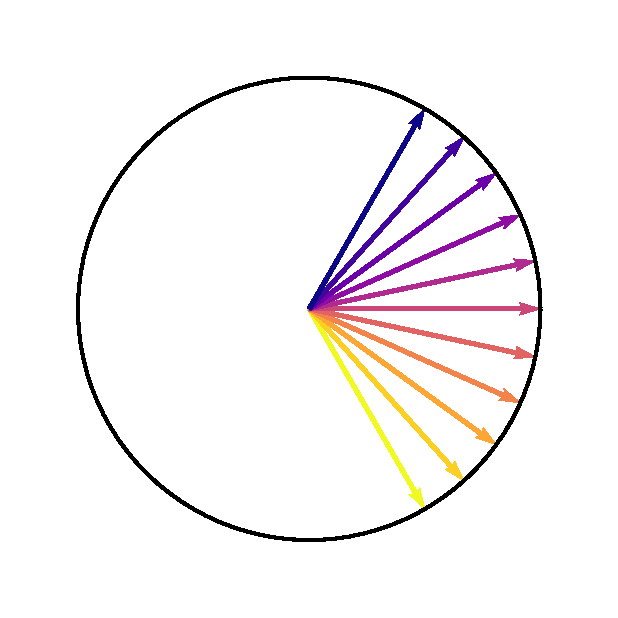
\includegraphics[width=1\textwidth]{Theory/SE/se_spins_t_te_inverted.eps}
		\caption{After 180\degree{ } pulse}
		\label{fig:theory_se_spins_t_te_by_2_inverted}
	\end{subfigure}
	\begin{subfigure}[c]{0.24\textwidth}
		\centering
		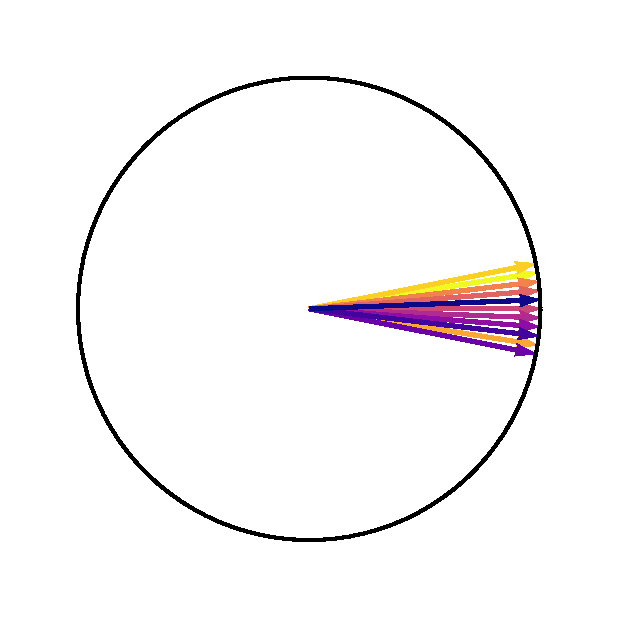
\includegraphics[width=1\textwidth]{Theory/SE/se_spins_t_2te.eps}
		\caption{$t$ = 2TE}
		\label{fig:theory_se_spins_t_te}
	\end{subfigure}
	\caption{Spins evolving in a spin echo sequence showing the de-phasing, (\subref{fig:theory_se_spins_t_te_by_2}), refocusing pulse, (\subref{fig:theory_se_spins_t_te_by_2_inverted}), and subsequent refocusing, (\subref{fig:theory_se_spins_t_te}).}
	\label{fig:theory_se_spins}
\end{figure}

By repeating this sequence over a range of \ac{TE} the \ttwo curve can be samples and fit to \eqref{eq:theory_bloch_transverse_mxy} to estimate \ttwo and $M_{xy0}$. The \ac{SE} sequence is the most basic form of \ttwo mapping, more methods are explored and compared in Chapter \ref{chap:t2_mapping}.

\subsection{Optimisation of Tissue Contrast}
Quantitative mapping of \tone, \ttwo and \ttwostar can often be a slow process due to the number of acquisitions required at different time points to sample relaxation curves. Often it is more desirable to acquire a volume at a single time with the intensity difference between tissues of interest maximised. Although the voxel intensities do not directly represent any quantitative underlying physical properties of the tissue, the contrast between tissues is sufficient for diagnosis or further analysis.
\begin{figure}[H]
	\centering
	\includegraphics[width=0.8\textwidth]{Theory/Tissue_Contrast/tissue_contrast.eps}
	\caption{The signal generated from renal cortical and medullary tissues \cite{cox_multiparametric_2017} and difference between signals. This shows that the contrast between the two tissues is optimal if the \acf{TI} is 1500 ms.}
	\label{fig:theorgy_tissue_contrast}	
\end{figure}
\subsection{Diffusion Imaging}


\section{Forming an Image}

\newpage
\section{References}
\defbibheading{bibliography}[\refname]{}
\printbibliography